\chapter{Example Chapter}\label{ch:ExampleChapter}
	\lstset{style=LaTeXStyle}
	This chapter aims to provide examples how how to structure and create specific components in your thesis document.
	Throughout this section, \LaTeX's automatic placement for figures and tables will be disabled in most cases.
	This is being done to add a specific flow to \textbf{THIS DOCUMENT}; this should be avoided in one's thesis as it can lead to poor placement of figures, tables, and other \enquote{floats}, as well as cause unnecessary white space.
	\section{General Text Layouts}
		\subsection{Lists}
			\LaTeX{} has a few built-in ways for handling lists.
			The three that we will be looking at here (formatted in an enumerated list) are:
			\begin{enumerate}
				\item \lstinline|enumerate|
				\item \lstinline|itemize|
				\item \lstinline|description|
			\end{enumerate}
			These each create lists in a slightly unique way.
			And all of these lists can be nested in each other.
			For \path{enumerate}, this creates a numbered list, where each level has a different style of \enquote{numbered list}.
			\begin{enumerate}
				\item First Item
					\begin{enumerate}
						\item First Sub Item
							\begin{enumerate}
								\item First Sub Sub Item
								\item Second Sub Sub Item
							\end{enumerate}
						\item Second Sub Item
					\end{enumerate}
				\item Second Item
			\end{enumerate}
			For \path{itemize}, this creates a non-numbered list.
			Every level that is created will have a different style bullet.
			\begin{itemize}
				\item First Item
					\begin{itemize}
						\item First Sub Item
							\begin{itemize}
								\item First Sub Sub Item
								\item Second Sub Sub Item
							\end{itemize}
						\item Second Sub Item
					\end{itemize}
				\item Second Item
			\end{itemize}
			For \path{description}, this creates a descriptive list.
			Descriptions should have the optional argument included for each \lstinline|\item| otherwise the line will have a blank in the beginning like the \textit{Second Item} in the next list and not align with the other items.
			\begin{description}
				\item[LVL1] First Item
					\begin{description}
						\item[LVL1-1] First Sub Item
							\begin{description}
								\item[LVL1-1-1] First Sub Sub Item
								\item[LVL1-1-2] Second Sub Sub Item
							\end{description}
						\item[LVL1-2] Second Sub Item
					\end{description}
				\item Second Item
			\end{description}
			Beyond the previous examples, there are no limitation on the types of lists that are nested, allowing for combined styles as shown in the following list.
			\begin{enumerate}
				\item First Item
					\begin{itemize}
						\item First Sub Item
							\begin{description}
								\item[LVL1-1-1] First Sub Sub Item
								\item[LVL1-1-2] Second Sub Sub Item
							\end{description}
						\item Second Sub Item
					\end{itemize}
				\item Second Item
			\end{enumerate}
		\subsection{Footnotes}
			\LaTeX{} can have footnotes added in very easily. 
			Generally these footnotes will be inserted in one of two ways.
			Using the in-line command:
			\begin{Center}
				\lstinline|\footnote{footnote text}|\footnote{footnote text} 
			\end{Center}
			Or by using the split footnote.
			For a split footnote, the macro:
			\begin{Center}
				\lstinline|\footnotemark[n]|\footnotemark{}
			\end{Center}
			is used to indicate where the mark should be inserted.
			And the macro: 
			\begin{Center}
				\lstinline|\footnotetext[n]{split footnote text}|.
			\end{Center}
			is used to signify what the text for the indicated foot note should be.
			This allow you to help keep your document more organized with the drawback that it is the user's responsibility to keep track of the foot note numbers or ensure that a \lstinline|footnotemark| is followed by it's corresponding \lstinline|footnotetext|.
			For this reason, I recommend using the in-line footnotes.
		
			\footnotetext{split footnote text}
		
	\section{Cross-References and Citations}\label{sec:citref}
		This section will be showing off some of the different ways to include \enquote{citations} and \enquote{cross-references} within your document.
		Note that \textbf{cross-references} in \LaTeX{} utilize \lstinline|\ref{}| as a command, while one might think that this is short for reference this is not the case citation/references utilize the \lstinline|\cite{}| commands.
	  
		\subsection{Cross-References}\label{subsec:cross-reference}
			In \LaTeX{}, references will \enquote{reference} a \lstinline|\label{Reference:Label}| command. 
			This section has the following command to define the the section:
			\begin{Center}
				\lstinline|\section{Citations and References}\label{sec:citref}|
			\end{Center}
			By using \lstinline|\ref{sec:citref}|, this allows you to insert a reference that look like this: \ref{sec:citref}.
			Now this by itself is not the most useful, to make it a bit better we should keep track of what we are referencing, in this case a \textbf{Section}, and add this label in front of the reference (\lstinline|Section~\ref{sec:citref}|) and this will display like this: Section~\ref{sec:citref}.
			Note to ensure the reference is not split we add a non-breaking space (\lstinline|~|) to prevent \LaTeX{} from adding a linebreak.

			While using the ref command, you might ask \enquote{\textit{Why does \LaTeX{} not just know what it is that I am referencing and insert that automatically in front of the reference?}}
			The answer is to provide more flexibility to the user.
			However, that being said, individuals have created a number of packages that work to enhance the workflow of adding these cross-references.
			Some of these are provided by the \textbf{hyperref} and \textbf{cleveref} packages.
			To include these packages add the following lines to the bottom of your preamble (order matters, cleveref needs to be after hyperref and hyperref should be one of the last packages loaded):
			\begin{lstlisting}[style=LaTeXStyle]
				\usepackage{hyperref}
				\usepackage[nameinlink]{cleveref}
			\end{lstlisting}
			With these packages installed we can now use the commands in \Cref{tab:reftable}.\footnote{Note that becase the floats are added where they are in the text this causes them to insert large amounts of white space because it only fits on the following page.}
      \begin{table}[H]
        \caption{Built-in, hyperref, and cleveref commands and outputs}\label{tab:reftable}
        \centering
        \begin{tabularx}{0.5\textwidth}{CC} 
          \toprule
            \textbf{Command} & \textbf{Output} \\
          \midrule
            \multicolumn{2}{c}{built-in}\\
            \lstinline|\\ref\{\}|           & \ref{tab:reftable} \\
            \lstinline|\\pageref\{\}|       & \pageref{tab:reftable} \\
          \midrule
            \multicolumn{2}{c}{hyperref}\\
            \lstinline|\\autoref\{\}|       & \autoref{tab:reftable} \\
            %\lstinline|\\autoref*\{\}|      & \autoref*{tab:reftable} \\
          \midrule
            \multicolumn{2}{c}{cleveref}\\
            \lstinline|\\cref\{\}|          & \cref{tab:reftable} \\
            \lstinline|\\Cref\{\}|          & \Cref{tab:reftable} \\
            \lstinline|\\cref*\{\}|         & \cref*{tab:reftable} \\
            %\lstinline|\\Cref*\{\}|         & \Cref*{tab:reftable} \\
            \lstinline|\\cpageref\{\}|      & \cpageref{tab:reftable} \\
            \lstinline|\\Cpageref\{\}|      & \Cpageref{tab:reftable} \\
            \lstinline|\\namecref\{\}|      & \namecref{tab:reftable} \\
            \lstinline|\\nameCref\{\}|      & \nameCref{tab:reftable} \\
            %\lstinline|\\lcnamecref\{\}|    & \lcnamecref{tab:reftable} \\
            %\lstinline|\\labelcref\{\}|     & \labelcref{tab:reftable} \\
            %\lstinline|\\labelcpageref\{\}| & \labelcpageref{tab:reftable} \\
          \bottomrule
        \end{tabularx}
        \end{table}
        Further, the \textbf{cleveref} also includes features that allows for the auto sorting and combining of references:
        
        \begin{lstlisting}[style=LaTeXStyle]
			\Cref{fig:doubleImage,fig:singleImage,fig:tripleImage1,fig:quadImage}
		\end{lstlisting}
        
    Noting that there are \textbf{NO} spaces between the labels; this will produce: \Cref{fig:doubleImage,fig:singleImage,fig:tripleImage1,fig:quadImage}. Allowing one to quickly and efficiently keep references up-to-date and consistent in their style.
    More examples of the use of the \textbf{cleveref} cross-referencing is found through the rest of this \nameCref{ch:ExampleChapter}.
  \subsection{Citations}\label{subsec:citations}
      Citations are a lot easier than dealing with the cross-referencing.
      There are no additional packages required for citations, the built-in ones are feature-rich enough.
      Now, while there are no additional packages required to make citations in your document, there are in fact a few programs that should help you manage all of your citations/references.
      These programs can include Mendeley, JabRef, or Zotero; a comparison of the softwares can be found in \Cref{tab:refSoftware}, and more information of the use of JabRef can be found in \Cref{ch:JabRef}.
      
      \begin{table}[htbp]
          \centering
          \caption{Comparison of Reference Softwares}\label{tab:refSoftware}%
            \begin{tabularx}{0.9\textwidth}{Lcccr}
                \toprule
                    Software & Developer & Version & Free & License \\
                \midrule
                    JabRef   & The JabRef Team & 5.11   & Free   & MIT \\
                    Mendeley & Elsevier          & 2.99.0 & {Free up to 2 GB} & Proprietary \\
                    Zotero   & CDS               & 6.0.27 & {Free  up to 300 MB} & AGPL \\
                \bottomrule
            \end{tabularx}%
      \end{table}%
      
      Single citations can be included with the \lstinline|\cite{citationKey}| command, the one at the end of this sentence is created with the \lstinline|\cite{TEST}| command\cite{TEST}. 
      Multiple citations can be included in a single cite command by adding commas in between the citation keys. The citation at the end of this sentence shows how to create more than one citation and how they are grouped together, it is created with the \lstinline|\cite{testone,cite2,cite3,cite4,cite5}| command\cite{testone,cite2,cite3,cite4,cite5}.
      Finally this sentence shows how a gap in the citations is handled, this is created with the \lstinline|\cite{testone,cite2,cite3,cite5}| command\cite{testone,cite2,cite3,cite5}. 
  \section{Tables}
  Within this section we will explore some of the typical uses for a table, how to create them, and how to create a consistent look throughout your thesis.
  \LaTeX{} provides the default floats environment \path{table} that can be combined with the \path{tabular} environment to create tables in your works. 
  While these tables are functional they have a very plain look and feel to them.
  The package \path{tabularx} can be combined with the \path{booktabs} package to create elegant and consistent looking tables.
  A direct comparison of a standard table and the \path{tabularx} with \path{booktabs} can be seen in \Cref{tab:tableComparison}.
  \begin{table}[H]
    \caption{Tabular vs. Tabularx Comparison}\label{tab:tableComparison}
    \centering
    \begin{subtable}{0.45\textwidth}
        \caption{}\label{tab:tableComparison:b}
        \begin{tabular}{lcr} 
          \hline
            \textbf{Left} & \textbf{Centre} & \textbf{Right}\\%
          \hline
            Left Column & Centre Column & Right Column \\%
          \hline
        \end{tabular}
    \end{subtable}
    ~
    \begin{subtable}{0.45\textwidth}
        \caption{}\label{tab:tableComparison:a}
        \begin{tabularx}{\textwidth}{LCR} 
          \toprule
            \textbf{Left} & \textbf{Centre} & \textbf{Right}\\
          \midrule
            Left Column & Centre Column & Right Column \\
          \bottomrule
        \end{tabularx}
    \end{subtable}
  \end{table}
  As can be see in \Cref{tab:tableComparison}, well maybe not due to the overlap... the included \path{tabular} environment in \LaTeX{} does not restrict a table to being a specific size; it is completely up to the user to determine if a table will overflow, and, if it does, to break or change the layout to make the data fit.
  On the other hand, the \path{tabularx} package allows us to set the width of the table and inform it which columns should be scaled to fit the the data and the \path{tabularx} package will handle the heavy lifting for us.
  Thus creating a table that, first, fits in the space one specifies and, secondly, re-flows the data to fit the cells rather than running the contents into neighbouring content or into the margins and off the page.
  
  \path{Tabularx} uses similar formats to the tabular environment, except there is an additional column type: \path{X}.
  This column type, or one of the derivative column types shown below, must be included in the use of a \path{tabularx} table. 
  Failing to do so will cause an error. The additional column types that one might like to create for use with the \path{tabularx} environment are as follows:
  \begin{itemize}
    \item \textbf{C} - Centred Auto Sizing Column\\\lstinline|\newcolumntype{C}{>{\centering\arraybackslash}X}|
    \item \textbf{L} - Left Justified Auto Sizing Column \\\lstinline|\newcolumntype{L}{>{\raggedright\arraybackslash}X}|
    \item \textbf{R} - Right Justified Auto Sizing Column \\\lstinline|\newcolumntype{R}{>{\raggedleft\arraybackslash}X}|
  \end{itemize}
  
  \begin{table}[H]
    \caption{This is a basic table}
    \centering
    \begin{tabularx}{0.75\textwidth}{LCR} 
      % Equally spaced cells that are left, centre, and right aligned. 
      % The entire table will be 75% the width of the text.
      \toprule
        \textbf{Left Aligned Title} & \textbf{Centred Title} & \textbf{Right Aligned Title} \\
      \midrule
        This is left aligned & This is centred & This is right aligned\\
        This is left aligned & This is centred & This is right aligned\\
        This is left aligned & This is centred & This is right aligned\\
        This is left aligned & This is centred & This is right aligned\\
      \bottomrule
    \end{tabularx}
    \label{tab:basicTable}
  \end{table}
  In the following table, \Cref{tab:complexTable}, we use the \path{multirow} and \path{multicol} packages.
  These two packages allow one to merge cells together in a table.
  Beyond this, to include lines, the \lstinline|\cmidrule(l{<length>}r{<length>}){start_cell-end_cell}| from the \path{booktabs} package is used.
  To add a bit of a cleaner look the lines can be trimmed by including the \path{l{<length>}} or \path{r{<length>}} in the round brackets to trim the lines by the specified length for the left and right sides, respectively.
  Note that both line trim specifications do not need to be specified, in-fact one or none can be provide if the line does not need to be trimmed, \textit{e.g.}, \lstinline|\cmidrule{1-5}| or \lstinline|\cmidrule(r{3em}){2-3}|.
  \begin{table}[H]
    \caption{This is a complex table.}
    \centering
    \begin{tabularx}{0.95\textwidth}{lCR}
      % Left most cell is fitted to the content.
      % The centre and right columns are equally spaced cells that are centre, and right aligned. 
      % The entire table will be 75% the width of the text.
      \toprule
      \multirow{2}{*}{\textbf{This is two row\quad}} & \multicolumn{2}{c}{\textbf{This is two columns}}\\
      \cmidrule(l{2em}){2-3} % \cmidrule draws a partial line across cells #-#
       & \textbf{Centred Title} & \textbf{Right Aligned Title} \\
      \midrule
      \multirow{2}{*}{This is two row} & This is centred & This is right aligned \\
       & This is centred & This is right aligned \\
      \cmidrule(r{2em}){1-1}
      \multirow{2}{*}{This is two row} & This is centred & This is right aligned \\
       & This is centred & This is right aligned \\
      \bottomrule
    \end{tabularx}
    \label{tab:complexTable}
  \end{table}
  
  \section{Figures}
  This section will provide examples of how to create figures, and different types of multi/sub-figures. 
  Additionally, if you have many figures in a section and they are bleeding too much into the following sections a \lstinline|\clearpage| command can be issued before the next section. 
  However, note that this will force the next section to begin on a new page. 
  Note that the first \enquote{figure} is actually a \textbf{plate}; a plate is the proper title associated with a \textit{photograph}, however, is not always used in every department... if your are unsure ask your supervisor if the use of plates is common. Using the environment \path{plate} instead of \path{figure} and command \lstinline|\listofplates| will generate everything for you.
  \begin{plate}[H]
    \centering
    \includegraphics[width=0.7\textwidth]{example-image}
    \caption{This is an example of a single image plate.}
    \label{plate:singleImage}
  \end{plate}
  
  \begin{figure}[H]
    \centering
    \includegraphics[width=0.7\textwidth]{example-image}
    \caption{This is an example of a single figure.}
    \label{fig:singleImage}
  \end{figure}
  \begin{figure}[H]
    \centering
    \begin{subfigure}{0.45\textwidth}
      \includegraphics[width=\textwidth]{example-image}
      \caption{} % Leave blank for just letter
      \label{fig:doubleImage:a}
    \end{subfigure}
    ~
    \begin{subfigure}{0.45\textwidth}
      \includegraphics[width=\textwidth]{example-image}
      \caption{} % Leave blank for just letter
      \label{fig:doubleImage:b}
    \end{subfigure}
    \caption{This is an example of a double image figure.}
    \label{fig:doubleImage}
  \end{figure}
  
  \begin{figure}[H]
    \centering
    \hspace*{\fill}% Adds space to left of top image (prevents two images from going to top)
    \begin{subfigure}{0.45\textwidth}
      \includegraphics[width=\textwidth]{example-image}
      \caption{} % Leave blank for just letter
      \label{fig:tripleImage1:a}
    \end{subfigure}
    \hspace*{\fill} % Adds space to right of top image (prevents two images from going to top)
    \par\vspace{1em}% Adds space between upper and lower images
    \begin{subfigure}{0.45\textwidth}
      \includegraphics[width=\textwidth]{example-image}
      \caption{} % Leave blank for just letter
      \label{fig:tripleImage1:b}
    \end{subfigure}
    ~ % Adds space between the two lower figures
    \begin{subfigure}{0.45\textwidth}
      \includegraphics[width=\textwidth]{example-image}
      \caption{} % Leave blank for just letter
      \label{fig:tripleImage1:c}
    \end{subfigure}
    \caption{This is an example of a triple image figure.}
    \label{fig:tripleImage1}
  \end{figure}
  
  \begin{figure}[H]
    \centering
    \hspace*{\fill}% Adds space to left of top image (prevents two images from going to top)
    \begin{subfigure}{0.90\textwidth+1em} % 0.9 = 0.45 + 0.45, and 1em is the width of ~
      \includegraphics[width=\textwidth]{example-image}
      \caption{} % Leave blank for just letter
      \label{fig:tripleImage2:a}
    \end{subfigure}
    \hspace*{\fill} % Adds space to right of top image (prevents two images from going to top)
    \par\vspace{1em}% Adds space between upper and lower images
    \begin{subfigure}{0.45\textwidth}
      \includegraphics[width=\textwidth]{example-image}
      \caption{} % Leave blank for just letter
      \label{fig:tripleImage2:b}
    \end{subfigure}
    ~ % Adds space between the two lower figures
    \begin{subfigure}{0.45\textwidth}
      \includegraphics[width=\textwidth]{example-image}
      \caption{} % Leave blank for just letter
      \label{fig:tripleImage2:c}
    \end{subfigure}
    \caption{This is a second example of a triple image figure.}
    \label{fig:tripleImage2}
  \end{figure}
  
  \begin{figure}[H]
    \centering
    \begin{subfigure}{0.45\textwidth}
      \includegraphics[width=\textwidth]{example-image}
      \caption{} % Leave blank for just letter
      \label{fig:quadImage:a}
    \end{subfigure}
    ~ % Adds space between the two top figures
    \begin{subfigure}{0.45\textwidth}
      \includegraphics[width=\textwidth]{example-image}
      \caption{} % Leave blank for just letter
      \label{fig:quadImage:b}
    \end{subfigure}
    \par\vspace{1em} % Adds space between upper and lower images
    \begin{subfigure}{0.45\textwidth}
      \includegraphics[width=\textwidth]{example-image}
      \caption{} % Leave blank for just letter
      \label{fig:quadImage:c}
    \end{subfigure}
    ~ % Adds space between the two lower figures
    \begin{subfigure}{0.45\textwidth}
      \includegraphics[width=\textwidth]{example-image}
      \caption{} % Leave blank for just letter
      \label{fig:quadImage:d}
    \end{subfigure}
    \caption{This is an example of a quad image figure.}
    \label{fig:quadImage}
  \end{figure}
  
  \clearpage % forces the remaining images (floats to be placed)
  \section{Graphs \& Plots}
  In the following section there will be a few examples of how to generate plots.
  For more information on how to create plots, \href{https://mirror.its.dal.ca/ctan/graphics/pgf/contrib/pgfplots/doc/pgfplots.pdf}{\textcolor{blue}{\underline{here}}} is the manual for pgfplots.
  \begin{figure}[H]
    \centering
    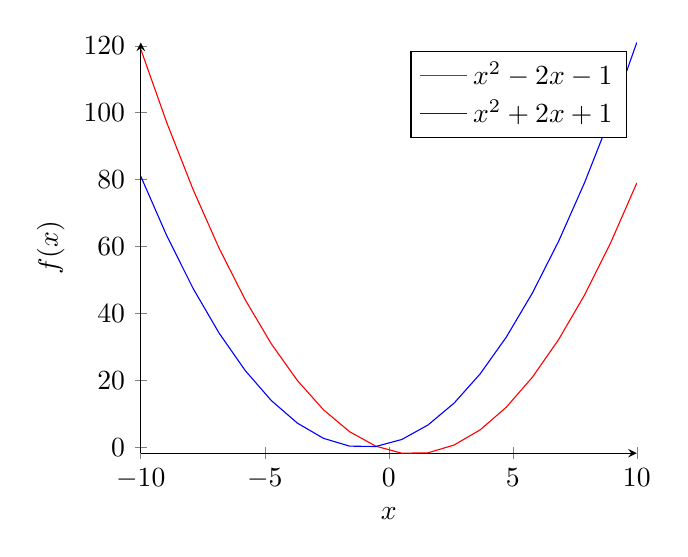
\begin{tikzpicture}
      \begin{axis}[
          width=0.65\textwidth,
          axis lines = left,
          xlabel = \(x\),
          ylabel = {\(f(x)\)},
      ]
        %Below the red parabola is defined
        \addplot [
            domain=-10:10, 
            samples=20, 
            color=red,
        ]
        {x^2 - 2*x - 1};
        \addlegendentry{\(x^2 - 2x - 1\)}
        %Here the blue parabola is defined
        \addplot [
            domain=-10:10, 
            samples=20, 
            color=blue,
            ]
            {x^2 + 2*x + 1};
        \addlegendentry{\(x^2 + 2x + 1\)}
      \end{axis}
    \end{tikzpicture}
    \caption{Plot of two parabola.}\label{fig:parabolaplot}
  \end{figure}
  
  \begin{figure}[H]
    \centering
    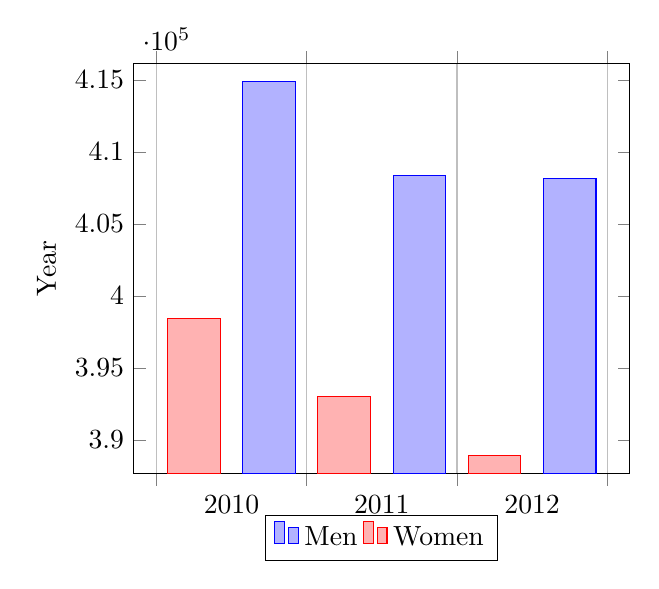
\begin{tikzpicture}
      \begin{axis}[
        width=0.65\textwidth,
        x tick label style={
          /pgf/number format/1000 sep=},
        ylabel=Year,
        enlargelimits=0.05,
        legend style={at={(0.5,-0.1)},
        anchor=north,legend columns=-1},
        ybar interval=0.7,
      ]
      \addplot 
        coordinates {(2012,408184) (2011,408348)
           (2010,414870) (2009,412156)};
      \addplot 
        coordinates {(2012,388950) (2011,393007) 
          (2010,398449) (2009,395972)};
      \legend{Men,Women}
      \end{axis}
    \end{tikzpicture}
    \caption{Example of a Bar Graph.}\label{fig:bargraph}
  \end{figure}
  
  \begin{figure}[H]
    \centering
    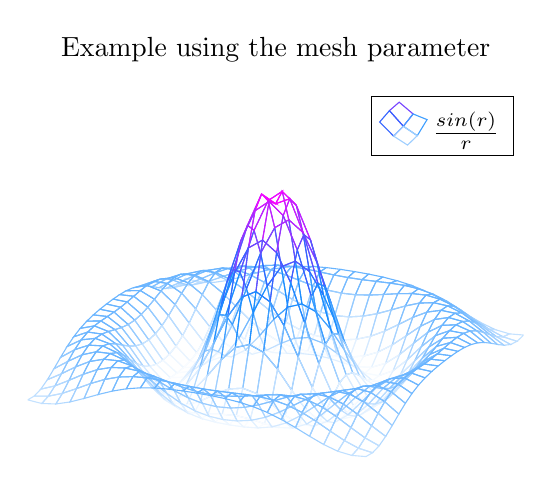
\begin{tikzpicture}
      \begin{axis}[
          width=0.65\textwidth,
          title=Example using the mesh parameter,
          hide axis,
          colormap/cool,
      ]
      \addplot3[
          mesh,
          samples=25,
          domain=-8:8,
      ]
      {sin(deg(sqrt(x^2+y^2)))/sqrt(x^2+y^2)};
      \addlegendentry{\(\frac{sin(r)}{r}\)}
      \end{axis}
    \end{tikzpicture}
    \caption{Example of a 3D Plot}\label{fig:3dplot}
  \end{figure}
  
  \begin{figure}[H]
    \centering
    \begin{tikzpicture}
      \begin{axis}[
          width=0.65\textwidth,
          enlargelimits=true,
      ]
      \addplot+[
          only marks,
          scatter,
          mark=*,
          mark size=2.9pt]
      table[meta=ma]
      {./02_Chapters/scattered_example.dat};
      \end{axis}
      \end{tikzpicture}
    \caption{Example of a Scatter Plot.}\label{fig:scatterplot}
  \end{figure}
  
  \clearpage
  \section{Equations}
  There are many ways to include formulas in your thesis. 
  This section will provide some different ways of adding them (inline and standalone), as well as provide some ways of referencing the equations.
  
  To start the simplest way to add an equation is using the built-in \LaTeX{} math mode. 
  To enter and exit math mode one just needs to use the \lstinline|\(<Equation>\)| symbols around an equation. While there also exists \lstinline|$<Equation>$| to add math, it is not recommended due to potential compatibility issues. Additionally, this, \lstinline|\(<Equation>\)|, method is capable of being redefined to add further customization. 
  An example of using math mode to get an inline equation is by using the following command:
  
	\begin{Center}
		\lstinline|\(\vec{F_{d}}=\frac{1}{2}\ A\ C_{d}\ \vec{V}^{2}\)|
	\end{Center}
  
  The above command has the effect of creating the following output: \(\vec{F_{d}}=\frac{1}{2}\ A\ C_{d}\ \vec{V}^{2}\).
  Sometimes it can be quite beneficial to separate what would be an in-line equation to be on its own line. for this we have two different ways of doing it. The first was will produce an equation that has no reference:
  
  \[
    E = m\ c^2
  \] % shorthand for the following way of writing equations.
  \begin{equation*}
    E = m\ c^2
  \end{equation*}
  The second will produce an equation with a reference. For this, there are two many ways of creating the reference, the first one, see \Cref{eq:Eq}, creates a numbered reference, the other one, see \Cref{eq:customTag}, creates a reference with a `tag'. The difference between the two is just the inclusion of a \lstinline|\tag{<text>}| command that will replace the regular number with \path{<text>}.
  \begin{equation}\label{eq:Eq}
    \pi = 3.1415...
  \end{equation}
  \begin{equation}\tag{Constant pi}\label{eq:customTag}
    \pi = 3.1415...
  \end{equation}
  
  If you have multiple equations that you want arranged very neatly, use the align environment and you can assign individual equations numbers as shown in \Cref{eq:multiref:a,eq:multiref:b,eq:multiref:c}.
  \begin{align}%Note: Alignment happens at the "=" character
    \label{eq:multiref:a} Equation1 & = 1\\
    \label{eq:multiref:b} Equation2 & = 2 + 2\\
    \label{eq:multiref:c} Equation3 & = 3 + 3 + 3
  \end{align}
  
	\section{Math}
		
		
		\begin{table}
			\begin{tabularx}{0.85\textwidth}{CCCCCC}
				\alpha
			\end{tabularx}
		\end{table}
  
    It may be very important in a math heavy thesis to be able to show your equations, or even data in a readable way. For this, we will explore some of the ways to create specific data.
    
        \subsection{Vector, Sets, Piecewise Functions, Matrix Math, and More}
        
        \begin{equation}
            \text{f}(x) = 
                \begin{cases}
                    x^{2*\ln{x}},&\text{if }x<3\\
                    -\frac{x}{2},&\text{if }3\leq{}x\leq{}4\\
                    x,&\text{if }4<x
                \end{cases}
        \end{equation}
        
        Vectors and Matrices are used in many fields of math and science and provide a convenient way to represent 2-Dimensional arrays of numbers.
            \begin{align}
                x&\in{}\left\{1,2,3,4,5,6,7\right\}\\
                V_{1} &= {\left(
                \begin{array}{cccc}
                    a, & b, & c, & d\\
                \end{array}
                \right)}\\
                V_{2} &= \left(
                \begin{array}{c}
                    a \\
                    b \\
                    c \\
                    d \\
                \end{array}
                \right)\\
                M &= {\left[
                \begin{array}{cccc}
                    a & b & c & d\\
                    e & f & g & h\\
                    i & j & k & l\\
                    m & n & o & p\\
                \end{array}
                \right]}
            \end{align}

  \printreferences % Add a Reference Section to the end of the Chapter.
